\documentclass{prettytex/ox/mmsc-special-topic}

\setlength{\headheight}{19.53pt}
\setlength{\headsep}{1.8em}
\setlength{\belowcaptionskip}{-12pt}
\setminted{fontsize=\footnotesize}
\AfterEndEnvironment{minted}{\vspace*{-0.8cm}}
\renewcommand{\operatorcolor}{black}

\addbibresource{sources.bib}
\tikzexternalize[prefix=tikz/]

\newcommand{\topictitle}{
  Numerical Solution of an Electrochemical Cell Model \\
  \normalsize using Analytical Approaches, Finite Differences and a Spectral Method
}
\newcommand{\candidatenumber}{1072462}
\newcommand{\course}{Scientific Computing}

\title{\topictitle}
\author{Candidate \candidatenumber}
\date{\today}

\makenoidxglossaries
\newacronym{dc}{DC}{Direct Current}
\newacronym{ac}{AC}{Alternating Current}
\newacronym{ode}{ODE}{Ordinary Differential Equation}
\newacronym{pde}{PDE}{Partial Differential Equation}

% TODO: check that all \cL{...} are used on mappings and not values

\begin{document}
  \pagestyle{plain}
  \mmscSpecialHeader[casestudy]

  \begin{abstract}
    \label{abstract}
    In this project report we will review the central concepts utilised in the group work conducted to make progress in the \gls{pde} problem associated with the electrochemical model of a battery cell and present numerical results.
    \vspace*{0.2cm}

    \noindent
    \textbf{Our Goal:}
    Numerically obtain the solution $\{a(x, T), b(x, T)\}$ of
    \vspace*{-0.2cm}
    \begin{subequations}
      \begin{empheq}[left={\empheqlbrace}]{align}
        \label{eq:problem-pde-a} &\frac{\partial a}{\partial t} = D_a \frac{\partial^2 a}{\partial x^2}, & a: \R^+ \times [0, T] \mapsto [0, 1],\, T \in \R^+,\; D_a \in \R^+, \\
        \label{eq:problem-pde-b} &\frac{\partial b}{\partial t} = D_b \frac{\partial^2 b}{\partial x^2}, & b: \R^+ \times [0, T] \mapsto [0, 1],\, D_b \in \R^+,               \\
        \label{eq:problem-bcs} &a(\infty, t) = 1,\; b(\infty, t) = 0,                                  & \text{boundary conditions } \forall\, t \in [0, T]\,,               \\
        \label{eq:problem-ics} &a(x, 0) = 1,\;\; b(x, 0) = 0,                                          & \text{initial conditions }\forall\, x \in (0, \infty)\,,            \\
        \label{eq:problem-mass-conservation} &\frac{\partial a}{\partial x} + D \frac{\partial b}{\partial x} = 0 \,, & \text{ where } D := D_b / D_a
      \end{empheq}
    \end{subequations}
    and optionally, the further boundary condition $a(0, t) = 0$, which corresponds to \underline{Chronoamperometry} or $\frac{\partial a}{\partial x}\big|_{x=0} = I(t)$ which is set according to a special \underline{Linear Sweep Voltammetry} method with $I(t)$ given in \Cref{eq:current}.
    \vspace*{0.05cm}

    The Finite Difference schemes are implemented in MATLAB and Python, whereas the Spectral Method is implemented in C++ using \tschebfun.
  \end{abstract}

  \begin{figure}[H]
    \centering
    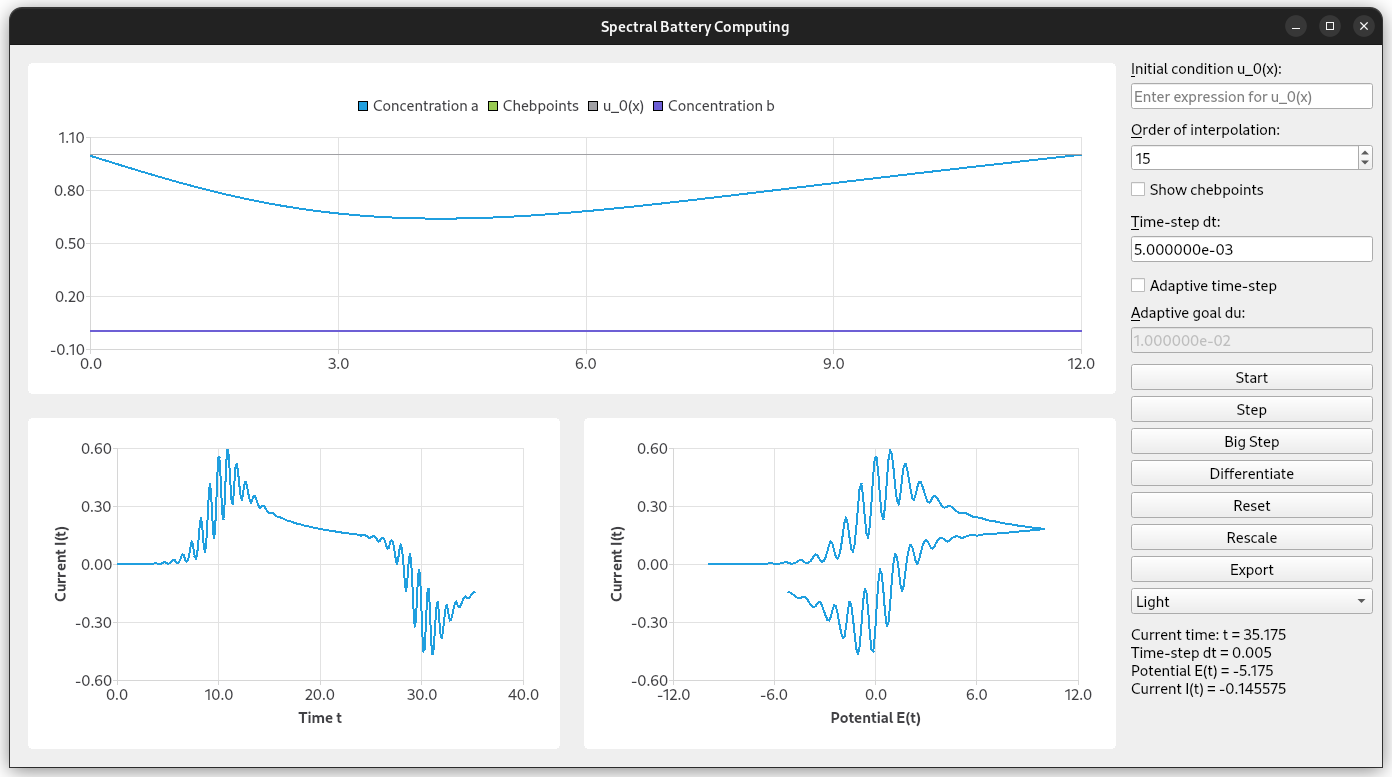
\includegraphics[width=\linewidth]{figures/screenshot.png}
    \caption{The Graphical User Interface of the Spectral Solver.}
  \end{figure}

  \pagebreak
  \pagestyle{normal}

  \section{Problem Introduction}
  \label{sec:introduction}
  Energy storage and its associated challenges are clearly among the most relevant questions today, not only for the industrial but also the public sector.
  Politically, many nations in the world are steering towards greener energy supplies.
  Renewable energy sources such as wind and sun usually have a fundamental issue, their availability is subject to an immense amount of fluctuation, which the energy grid must compensate through short- and long-term energy storage.

  Long-term solutions include for example pumped-storage hydroelectricity facilities, but these must be complemented with short-term storage approaches such as Lithium-Ion or Lithium-Iron-Phosphate ($\text{LiFePO}_4$) batteries.
  Of course, batteries also play a crucial role in customer end products such as smartphones or cars where mobility is a key requirement.
  Most modern batteries exploit electrochemical reactions to relate electrical potentials with chemical potentials and their associated difference ($\rightarrow$ voltage) and convert energy accordingly.
  The oxidation reaction we consider here is
  \begin{equation}
    A \leftrightarrow B + n e^-? \label{eq:oxidation-reaction}
  \end{equation}
  where $A$ and $B$ can be any chemicals and $n e^-$ represents $n$ electrons oxidated at the electrode surface \parencite{Gavaghan2000Jan}.

  \begin{figure}[H]
    \centering
    \inputtikz{battery-schema}
    \caption{Schematic representation of an electrochemical cell with the liquid solution of chemicals $A$ and $B$ in a container, together with an electrode where the oxidation reaction (\Cref{eq:oxidation-reaction}) takes place. For a small semi-minor axis length $R_y \ll H$ compared to the height of the container $H$ and a large eccentricity (so $R_x \gg R_y$), the 3-dimensional problem can be reduced to a two-dimensional one as depicted on the right-hand side.}
    \label{fig:battery-schema}
  \end{figure}

  The physical problem (cf. \Cref{fig:battery-schema}) in principle is three-dimensional but can be reduced down to two spatial dimensions, and even further down to one dimension when the electrode covers the entire ``floor'' of the container.
  As stated on \Cpageref{abstract}, this results in a coupled system of diffusion \gls{pde}s of the concentration functions $a$ and $b$, cf. \Crefrange{eq:problem-pde-a}{eq:problem-mass-conservation} in an infinitely large container.
  In practice, the container is modelled as large enough with length $L$ chosen in a way that does not make a large difference for the numerical solution.
  The electrode is located at $x = 0$ and the chemicals expand all the way to $x \rightarrow \infty$ or in practice, $x = L$.

  The initial conditions are that the chemical $A$ is present everywhere at $t=0$ while the chemical $B$ is not, so $a(x, 0) = 1$ and $b(x, 0) = 0$.
  The boundary conditions on the right (at $x \rightarrow \infty$) are motivated by the infinite size of the container, so a diffusion-type reaction will never fully propagate to the very end (right-hand side) of the container and hence we have that $a(x\rightarrow\infty, t) = 1$ and $b(x\rightarrow\infty, t) = 0$ in accordance with the initial conditions.

  Last but not least, \Cref{eq:problem-mass-conservation} describes mass conservation within the container - the flux of chemical $A$ must exactly cancel that of chemical $B$. This turns the differential equations into a coupled system.

  As mentioned above, we will consider three different cases that determine the behaviour of the system of \gls{pde}s: Chronoamperometry, Linear Sweep Voltammetry and Sine Wave Voltammetry.

  \subsection{Chronoamperometry}
  Chronoamperometry is an analytical technique employed in electrochemistry to study the internals of a working electrode. In this case, we consider a potential function $E(t)$ with a large step located at the surface of the electrode.
  The step is modelled as large enough to force the left-hand boundary condition
  \begin{equation}
    a(x=0, t) = 0 \quad\text{ and }\quad b(x=0, t) = 1\,.
    \label{eq:chrono-bc}
  \end{equation}
  Note that this conflicts with the initial condition for $a$ which is 1 everywhere at $t = 0$, and similarly for $b$ it is 0 everywhere at $t = 0$.
  This conflict causes a large jump in the solution (as we will see later, the similarity solution approach yields $\approx \erf\left(\frac{x}{2 \sqrt{D_a t}}\right)$ whose argument explodes to $\infty$ at $t = 0$ and then slowly recovers).
  That is not a problem for finite difference schemes, but a large issue for spectral methods in polynomial bases as they cannot encode a jump in their expansion with finite coefficients.

  \subsection{Linear Sweep Voltammetry}
  Linear sweep voltammetry is another method to study a working electrode, by sweeping the potential $E(t)$ linearly in time. In our case, this is done by
  \begin{equation}
    E_{dc}(t) = \begin{cases}
      E_{start} + t                     & \text{ when } 0 \leq t< t_{rev},           \\
      E_{start} + t_{rev} - (t-t_{rev}) & \text{ when } t_{rev} \leq t\leq 2t_{rev}.
    \end{cases}
    \label{eq:linear-potential}
  \end{equation}
  with parameters $E_{start} = -10$ and $t_{rev} = 20$.
  In the case of linear sweep voltammetry, we take the potential $E(t) = E_{dc}(t)$, the \gls{dc} potential.

  We then study the current $I(t)$ as the following function of the potential
  \begin{equation}
    I(t) = \kappa_0 \left(a \e^{(1-\alpha) (E(t) - E_0)} - b \e^{-\alpha (E(t) - E_0)}\right)_{x=0}
    \label{eq:current}
  \end{equation}
  with parameters $\kappa_0 = 35$ and $E_0 = 0$.
  Note that this expression depends on the values of $a$ and $b$ at $x = 0$, so the concentrations of $A$ and $B$, respectively, at the electrode.

  \subsection{Sine Wave Voltammetry}
  Sine wave voltammetry is a small extension to linear sweep voltammetry, where we add a small harmonic perturbation on top of the \gls{dc} potential $E_{dc}$, which altogether we will refer to as the \gls{ac} potential:
  \begin{equation}
    E(t) = E_{dc}(t) + \Delta E \sin(\omega t)\,.
    \label{eq:ac-potential}
  \end{equation}

  We will refer to linear sweep and sine wave voltammetry together as cyclic voltammetry.

  In the following, we will introduce necessary mathematical background on Laplace transforms and Chebyshev polynomials (\Cref{sec:math-background}), obtain an analytical solution using a similarity solution and Laplace-transform approach in \Cref{sec:analytical-approaches}, discuss the finite difference scheme one can use to solve the problem numerically in \Cref{sec:finite-differences} and finally introduce the Chebyshev spectral method used for most results in this report (\Cref{sec:spectral-method}).

  \pagebreak
  \section{Mathematical Background}
  \label{sec:math-background}
  Let $\N$ denote the nonnegative integers, so $0 \in \N$.
  Similarly, let $\R^+ = [0, \infty)$ denote the nonnegative real numbers.

  \subsection{The Laplace Integral Transform}
  This subsection will provide a short introduction of the Laplace transform and state theorems necessary for later treatment. What is the Laplace transform?
  A near-bijective, \emph{linear} integral transformation from one function space to another, cf. \Cref{def:laplace}.
  The mapping is injective, as given by Lerch's theorem. Surjectivity of the transformation is a more delicate matter and does not always hold.
  However, for most practical use-cases the transformation is one-to-one.
  Even if so, bijectivity would only hold up to differences on a subset of the domain of measure zero (so when two functions are equal \textit{almost everywhere}).

  \begin{definition}{Laplace Integral Transform}{laplace}
    Given a function $a: \R \mapsto \R$, its Laplace transform $\hat{a}: \C \mapsto \C$ is given by
    $$\hat{a}(s) = \cL\{a\}(s) := \int_{0}^{\infty} a(t) \e^{-st} \,\ddt\,.$$
  \end{definition}

  A notation commonly employed in the context of signal processing is $a(t) \;\laplace\; \hat{a}(s)$ to signify a \textit{transformation pair}, so
  $$a(t) \;\laplace\; \hat{a}(s) \quad\Longleftrightarrow\quad \hat{a}(s) = \cL\{t \mapsto a(t)\}(s)\,.$$
  In the following, we will mostly consider functions of two variables $a: \R \times \R \mapsto \R$ (the concentration of a chemical being a function of time $t \in \R$ and space $x \in \R$).
  In these cases, we are only transforming in one variable, namely $t$, and we will consider $x$ only as a parameter of the transformation pair.

  Laplace transforms are especially valuable for physical systems as many of them expose exponentially decaying and/or periodic behaviours which the Laplace transform is well-suited for due to the form of its kernel.
  Decaying behaviour is captured by the real component of the argument $s$, $\Re(s)$, whereas periodicities are captured by the imaginary part $\Im(s)$\footnote{Consider for comparision the Fourier transform $\cF(a)(\omega) := \int_{-\infty}^{\infty} a(t) \e^{\i \omega t} \,\ddt$ which captures periodic frequencies, where the kernel automatically follows multiplication along the unit circle due to the imaginary-valued exponent $\i\omega t$ (the argument $\omega \in \R$ is real-valued). Intuitively, the Laplace transform coincides with the Fourier transform if evaluated at $s = \i \omega$.}.

  In order to transform a function $\hat{a}$ from the frequency domain back to its original $a$ in the time domain, much like finding antiderivatives, one can use a lookup-table of known transformation pairs $a\;\laplace\;\hat{a}$ and harness the linearity of the Laplace transform $\cL$.
  For highly composite functions where tables cannot help, the inverse is given by Mellin's inverse formula which is also an integral.

  The most important result in the context of this report is the differentiation theorem, \Cref{thm:laplace-diff}, which we will only state here and use later.

  \begin{theorem}{Laplace Transform of the Derivative}{laplace-diff}
    Given a function $a(t)$ and a corresponding Laplace-transform $\hat{a}(s) = \cL\{a\}(s)$, the transform of the derivative $a'(t)$ of the original function is given by
    $$\cL\{a'\}(s) = \cL\left\{t \mapsto \frac{\partial a}{\partial t}\right\}(s) = s\hat{a}(s) - a_0\,,$$
    where $a_0 := a(t=0)$.
  \end{theorem}

  \begin{proof}
    From \Cref{def:laplace} directly, we have
    \begin{align*}
      \cL\{a'\}(s) & = \int_{0}^{\infty} a'(t) \e^{-st} \,\ddt = [a(t) \e^{-st}]_{t=0}^{\infty} + s \int_{0}^{\infty} a(t) \e^{-st} \,\ddt                                                                         \\
                   & = \underbrace{\lim_{t \rightarrow \infty} \left(a(t) \e^{-st}\right)}_{\rightarrow 0, \text{ as } s > 0 \text{ and } a \text{ grows slow}} - a(0) \e^{0} + s \cL\{a\}(s) = s\hat{a}(s) - a(0)
    \end{align*}
    using integration by parts. The upper boundary term as $t \rightarrow \infty$ vanishes because $s > 0$ and $a$ is assumed to grow slower than $\e^{-st}$.
  \end{proof}

  Another important result is the initial value theorem (\Cref{thm:initial-value}) which will later allow us to use a boundary condition of $a$ on the transformed $\hat{a}$.

  \begin{theorem}{Initial Value}{initial-value}
    For a function $a: \R \mapsto \R$ with corresponding Laplace-transform $\hat{a} = \cL\{a\}$,
    $$\lim_{s \rightarrow \infty} s \hat{a}(s) = \lim_{t \rightarrow 0^+} a(t)$$
    relates $a$'s \textit{initial value} with the transform evaluated at $s \rightarrow \infty$.
  \end{theorem}

  Highly relevant in signal processing and the theory of linear time-invariant systems, the convolution theorem (\Cref{thm:convolution-theorem}) allows us to rewrite a convolution of two functions as the product of their Laplace transforms.

  \begin{theorem}{Laplace Convolution}{convolution-theorem}
    Given two functions $a: \R \mapsto \R$ and $b: \R \mapsto \R$,
    $$\cL\{a * b\} = \cL\{a\} \cdot \cL\{b\}, \quad \text{ where }\quad (a * b)(t) = \int_{0}^{t} a(\tau) b(t-\tau)\,\ddt\,.$$
  \end{theorem}

  Similar results are available for the Fourier transform and other integral transforms.

  \subsection{Chebyshev Polynomials}
  In order to introduce the spectral method in \Cref{sec:spectral-method}, let us first define the basis in which the spectral method will operate - the basis of Chebyshev polynomials of the first kind (\Cref{def:chebpoly}).

  \begin{definition}{Chebyshev Polynomial of the First Kind}{chebpoly}
    \chebyshev\footnote{Named after Pafnuty Lvovich \chebyshev, alternatively transliterated as Tchebycheff, Tchebyshev (French) or \textsc{Tschebyschow} (German).} polynomials $T_k: \R \mapsto \R$ are functions satisfying
    \begin{align*}
      T_k(x) = T_k(\cos \theta) := \cos(k \theta) = \frac{1}{2} (z^k + z^{-k}) \\
      z := \e^{i \theta},\quad x := \Re(z) = \cos(\theta) = \frac{1}{2}(z + z^{-1})
    \end{align*}
    for degree $k \in \N$. Then, $T_0(x) = 1$, $T_1(x) = x$, $T_2(x) = 2x^2-1$, and so on.
  \end{definition}

  There are not only Chebyshev polynomials of the first kind, but also those of the second kind (\Cref{def:chebpoly2ndkind}) which we introduce in order to deduce a differentiation result we will use later in \Cref{sec:spectral-method}.

  \begin{definition}{Chebyshev Polynomial of the Second Kind}{chebpoly2ndkind}
    Chebyshev polynomials $U_k: \R \mapsto \R$ are functions satisfying
    \begin{align*}
      U_k(\cos \theta) \sin \theta := \sin\left((k+1) \theta\right)
    \end{align*}
    for degree $k \in \N$. Then, $U_0(x) = 1$, $U_1(x) = 2x$, $U_2(x) = 4x^2-1$, and so on.
  \end{definition}
  Note that Chebyhsev polynomials of the first and second kind fulfill the same recurrence relationship, $T_{k+1}(x) = 2x T_k(x) - T_{k-1}(x)$ and $U_{k+1}(x) = 2x U_k(x) - U_{k-1}(x)$. The difference between them arises from the second polynomial respectively which is $T_1(x)=x$ for the first kind and $U_1(x) = 2x = 2 T_1(x)$ for the second kind.

  Further note that $T_k(1) = T_k(\cos 0) = 1$, $T_k(-1) = T_k(\cos \pi) = \cos(k \pi) = (-1)^k$.
  Similarly, for the Chebyshev polynomials of the second kind,
  \begin{align}
    \label{eq:cheb2ndkind-critical-value-1} U_k(1)   & = U_k(\cos 0) = \lim_{\theta \rightarrow 0} \frac{\sin\left((k+1) \theta\right)}{\sin \theta} = \lim_{\theta \rightarrow 0} \frac{(k+1)\cos\left((k+1) \theta\right)}{\cos \theta} = (k+1)\,, \\
    \label{eq:cheb2ndkind-critical-value--1} U_k(-1) & = \lim_{\theta \rightarrow \pi} \frac{\sin\left((k+1) \theta\right)}{\sin \theta} = \lim_{\theta \rightarrow \pi} \frac{(k+1)\cos\left((k+1) \theta\right)}{\cos \theta} = (k+1) (-1)^k\,,
  \end{align}
  following directly from their \Cref{def:chebpoly2ndkind} and using de L'Hospital's rule to resolve the value of the $\frac{0}{0}$ situation.

  \section{Analytical Approaches}
  \label{sec:analytical-approaches}
  This section will consider a similarity solution and Laplace-transform approach to find analytical relationships between the solution and current.
  Note first of all that when $D = 1$, we have that $a + b = 1$ following from the mass conservation \Cref{eq:problem-mass-conservation}
  $$D = 1 \quad\Rightarrow\quad \frac{\partial}{\partial x} (a + b) = 0 \quad\Rightarrow\quad \text{integrate to get } a + b = \text{const}.\,,$$
  which we can combine with the initial conditions \Cref{eq:problem-ics} to find the constant equal to one and hence $a + b = 1\; \forall\; x\in[0, \infty), t\in\R$.

  \subsection{Similarity Solution}
  The diffusion equations \Cref{eq:problem-pde-a} and \Cref{eq:problem-pde-b} can be solved independently through a similarity solution approach.
  The idea behind the latter is to turn the \gls{pde} into an \gls{ode} by introducing a variable $\eta \in \R$ that depends on both other variables $x$ and $t$.
  For a diffusion-type equation, the correct ansatz would be letting
  $$a(x, t) = f(\eta), \quad \eta := \frac{x}{\sqrt{t}}\,,$$
  with $f: \R \mapsto \R$ and substituting back into \Cref{eq:problem-pde-a} accordingly.
  Respecting the chain rule on derivatives of $f$ accordingly, we arrive at
  $$\frac{\partial a}{\partial t} = -\frac{1}{2} x t^{-\frac{3}{2}} f'(\eta) = D_a \frac{\partial^2 a}{\partial x^2} = D_a t^{-1} f''(\eta)$$
  where we multiply both sides by $t$ to arrive at a simple form
  \begin{align}
    \label{eq:similarity-solution-ode} D_a f''(\eta) + \frac{1}{2} \eta f'(\eta) & = 0\,,
  \end{align}
  which can be solved by substituting $h(\eta) := f'(\eta)$ and solving $D_a \frac{\dd h}{\dd \eta} = \frac{-1}{2} \eta h(\eta)$ by separation of variables:
  $$\int\frac{\dd h}{h} = \frac{-1}{2D_a} \int \eta \,\dd\eta \quad \Rightarrow \quad \ln(h) = -\frac{\eta^2}{4D_a} + \tilde{c_1} \quad\Rightarrow\quad h(\eta) = c_1 \e^{\frac{-1}{4D_a}\eta^2}\,,$$
  which in turn may be integrated to get $f(\eta)$ and thereby $a(x, t)$,
  $$f(\eta) = c_1 \int \e^{\frac{-1}{4D_a}\eta^2} \dd\eta = c_1 \sqrt{D_a \pi} \erf\left(\frac{\eta}{2 \sqrt{D_a}}\right) + c_2\,.$$
  Substituting back, we get
  \begin{align}
    a(x, t) & = c_1 \sqrt{D_a \pi} \erf\left(\frac{x}{2 \sqrt{D_a t}}\right) + c_2\,, \\
    b(x, t) & = c_3 \sqrt{D_b \pi} \erf\left(\frac{x}{2 \sqrt{D_b t}}\right) + c_4\,,
  \end{align}
  where the solution of $b(x, t)$ is obtained by the same procedure.
  Using \Cref{eq:problem-bcs} and \Cref{eq:problem-ics} one can determine $$c_2 = 1 - \sqrt{D_a \pi} c_1\quad \text{ and }\quad c_4 = -\sqrt{D_b \pi} c_3\,.$$
  The spatial derivatives are given by
  $$\frac{\partial a}{\partial x} = c_1 \e^{-\frac{x^2}{4D_at}} t^{-\frac{1}{2}} \quad \text{ and }\quad \frac{\partial b}{\partial x} = c_3 \e^{-\frac{x^2}{4D_bt}} t^{-\frac{1}{2}}\,.$$
  Further considering the mass conservation equation $\frac{\partial a}{\partial x} + D \frac{\partial b}{\partial x} = 0$ (\Cref{eq:problem-mass-conservation}) which couples $a$ with $b$, one can derive a relation between $c_1$ and $c_3$,
  $$c_3 = -\frac{D_a}{D_b} \e^{\left(\frac{1}{D_b} - \frac{1}{D_a}\right) \frac{x^2}{4t}} c_1 = -\frac{D_a}{D_b} \e^{\frac{(D_a-D_b) x^2}{4t D_a D_b}} c_1\,.$$

  In the case of \underline{Chronoamperometry}, the constant $c_1$ is determined by letting
  $$a(x=0, t) = 0 \quad\Rightarrow\quad c_2 = 1 - \sqrt{D_a\pi} c_1 = 0 \quad\Rightarrow\quad c_1 = \frac{1}{\sqrt{D_a \pi}}\,,$$
  which then, using the spatial derivatives given above, leads us to a current of the form
  \begin{equation*}
    I(t) = \frac{\partial a}{\partial x}\bigg|_{x=0} = \frac{c_1}{\sqrt{t}} = \frac{1}{\sqrt{D_a \pi t}}\,,
  \end{equation*}
  whereas for \underline{Linear Sweep Voltammetry} the constant is determined by that very current
  $$\frac{\partial a}{\partial x}\bigg|_{x=0} = I(t) \quad\Rightarrow\quad c_1 = \sqrt{t} I(t) \text{ and } c_2 = 1 - \sqrt{D_a \pi t} I(t)\,.$$

  % TODO: maybe write down the full expressions? Is maths correct?
  % TODO: When $D = 1$, we have ...

  \subsection{Voltammetry Integral Equation}
  \subsubsection{Derivation using the Laplace Transform}
  As mentioned above, the Laplace Integral Transform is especially useful in the context of differential equations, mostly due to \Cref{thm:laplace-diff}.
  Applying it to our \textit{partial} differential diffusion equation \Cref{eq:problem-pde-a} transforms the problem into one of solving an \textit{ordinary} differential equation which is usually much easier.
  Similarly, \glstext{ode}s could be turned into algebraic equations using an analogous approach.

  Starting from \Cref{eq:problem-pde-a}, we Laplace-transform both sides and then apply \Cref{thm:laplace-diff} in time $t$ to arrive at
  \begin{align*}
    \frac{\partial a}{\partial t}                                   & = D_a \frac{\partial^2 a}{\partial x^2} \quad                             & \textcolor{gray}{\text{Laplace-transform w.r.t. } t} \\
    \cL\left\{t \mapsto \frac{\partial a}{\partial t}\right\}       & = D_a \cL\left\{t \mapsto \frac{\partial^2 a}{\partial x^2}\right\} \quad & \textcolor{gray}{\text{Use \Cref{thm:laplace-diff}}} \\
    s \hat{a}(s) - a_0(x)                                           & = D_a \frac{\partial^2 \hat{a}}{\partial x^2} \quad                       & \textcolor{gray}{\text{Rearrange}}                   \\
    \frac{\partial^2 \hat{a}}{\partial x^2} - \frac{s}{D_a} \hat{a} & = -\frac{a_0(x)}{D_a}
  \end{align*}
  where $\hat{a} := \cL\{a\}$ and $a_0(x) := a(x, t=0)$, which is a second-order constant-coefficient \glsdesc{ode} in space $x$. Its characteristic polynomial is $\lambda^2 + \frac{s}{D_a} = 0$ which, together with the initial condition $a_0 = 1$ and resulting particular solution $\hat{a}_p(x, s) = \cL\{-1\}(s) = \frac{1}{s}$\footnote{$\cL\{1\} = \int_{0}^{\infty} \e^{-st} \,\ddt = \frac{1}{s} \left[\e^{-st}\right]_0^\infty = \frac{-1}{s}$.}, leads us to the general solution
  \begin{equation}
    \hat{a}(x, s) = c_1 \e^{\sqrt{\frac{s}{D_a}}x} + c_2 \e^{-\sqrt{\frac{s}{D_a}}x} + \frac{1}{s D_a}\,,\quad c_1, c_2 \in \R\,.
    \label{eq:laplace-pre-solution}
  \end{equation}

  The constant $c_1$ then vanishes when applying the initial value theorem (\Cref{thm:initial-value})
  $$\lim_{s \rightarrow \infty} s \hat{a}(s) = \lim_{s \rightarrow \infty} \underbrace{c_1 s \e^{\sqrt{\frac{s}{D_a}}x}}_{\rightarrow \infty} + \underbrace{c_2 s \e^{-\sqrt{\frac{s}{D_a}}x}}_{\rightarrow 0} + 1 \overset{!}{=} \lim_{t \rightarrow 0^+} a(t) = 1$$
  because $c_1 \neq 0$ would cause its corresponding term to explode. Considering the other boundary condition of linear sweep voltammetry
  $$\frac{\partial a}{\partial x}\bigg|_{x=0} = I(t) \quad \Leftrightarrow \quad \frac{\partial \hat{a}}{\partial x} \overset{!}{=} \hat{I}(s) \quad \Leftrightarrow \quad c_2 \sqrt{\frac{s}{D_a}} \e^{0} = \hat{I}(s)\,,$$
  where $\hat{I}(s) := \cL\{I\}(s)$ and we obtain $c_2(s) = \frac{-\hat{I}(s)}{\sqrt{s}}$.
  So \Cref{eq:laplace-pre-solution} becomes
  \begin{equation}
    \hat{a}(x, s) = \frac{-\hat{I}(s)}{\sqrt{s}} \e^{-\sqrt{\frac{s}{D_a}}x} + \frac{1}{s D_a}\,,
    \label{eq:laplace-solution}
  \end{equation}
  which, evaluated at $x = 0$, becomes $\hat{a}(s, 0) = \frac{-\hat{I}(s)}{\sqrt{s}} + \frac{1}{s D_a}$, depending on the Laplace transform of the current $I(t)$.

  In principle, this is already a complete result in and of itself, as it provides the full solution on the entire domain in frequency-space \footnote{Frequency space is a term borrowed from Fourier analysis, where we say that the transformed functions reside in ``frequency space''. The usage is the same for Laplace's transformation.}. If one obtains the Laplace-transform of the current expression \Cref{eq:current} and performs the inverse transform of $\hat{a}$, even just numerically, the linear sweep voltammetry problem is solved in full as a similar procedure leads to the solution of the other concentration $b$.

  \subsubsection{At the Boundary}
  Within the scope of this report, we will consider an integral equation relating current $I(t)$ and the potential $E(t)$ to verify our numerical results.
  Inverse-transforming \Cref{eq:laplace-solution} at $x = 0$ where our boundary condition is given and using the convolution theorem (\Cref{thm:convolution-theorem}), we arrive at
  \begin{align*}
    a(x, t) = -\cL^{-1}\left\{s \mapsto \hat{I}(s) \cdot \hat{g}(s)\right\}(t) + \cL^{-1}\left\{s \mapsto \frac{1}{s D_a}\right\}(t) = -(I * g)(t) + \frac{1}{D_a}\,,
  \end{align*}
  where we introduced $\hat{g}(s) := \frac{1}{\sqrt{s}} = \cL\{g\}(s)$ the Laplace transfrom of $g(t) = \frac{1}{\sqrt{\pi t}}$.
  \begin{proof}
    $\cL\{t \mapsto \frac{1}{\sqrt{\pi t}}\}(s) = \frac{1}{\sqrt{\pi}} \int_0^\infty t^{-\frac{1}{2}} \e^{-st} \,\ddt = \frac{1}{\sqrt{\pi}} \int_0^\infty \cancel{t^{-\frac{1}{2}}} \e^{-su^2} \cancel{t^{\frac{1}{2}}}\,\ddu = \left[\erf(\sqrt{s} u) / \sqrt{s}\right]_0^\infty$ where we used a substitution $u = \sqrt{t}$ to resolve the product in the integrand, resulting in the Gaussian integral and subsequently, the error function $\erf(\sqrt{s}u)$ which satisfies $\erf(0) = 0$ and $\erf(\infty) = 1$ so the full transformation pair is $\frac{1}{\sqrt{\pi t}} \;\laplace\; \frac{1}{\sqrt{s}}$.
  \end{proof}

  \subsubsection{Simplification when $D = 1$ and $\kappa_0 \gg 1$}
  When $D = 1$, this results in the following expressions for $a(x=0, t)$ and $b(x=0, t)$,
  \begin{align}
    \label{eq:laplace-a} a(x=0, t) & = 1 - (I * g)(t) = 1 - \int_{0}^{t} \frac{I(\tau)}{\sqrt{\pi (t - \tau)}} \,\dd\tau\,, \\
    \label{eq:laplace-b} b(x=0, t) & = 1 - a(x=0, t) = \int_{0}^{t} \frac{I(\tau)}{\sqrt{\pi (t - \tau)}} \,\dd\tau\,,
  \end{align}
  which can be even further simplified when considering $\kappa_0 \gg 1$, where from \Cref{eq:current} we have the following relationship of $I(t)$, $E(t)$ and $b_0(t)$
  \begin{align*}
    I(t) & = \kappa_0 (1-b_0) \e^{(1-\alpha) V} - \kappa_0 b_0 \e^{-\alpha V} \\
         & = \kappa_0 \left[(1-b_0) \e^V - b_0\right] \e^{-\alpha V}          \\
         & = \kappa_0 \left[\e^V - (1+\e^V) b_0\right] \e^{-\alpha V}\,,
  \end{align*}
  where $V(t) := E(t) - E_0(t)$, $a_0 = a(x=0, t)$ and $b_0 = b(x=0, t)$.
  It can be further rearranged and simplified to yield an approximation to $b_0$,
  \begin{align*}
    \frac{I(t)}{\kappa_0 \e^{-\alpha V}} = \e^V - (1+\e^V) b_0 \quad \Leftrightarrow \quad
    b_0 = \frac{\e^V - \frac{I(t)}{\kappa_0 \e^{-\alpha V}}}{1+\e^V} \approx \frac{\e^V}{1 + \e^V} \quad \text{ when } \kappa_0 \gg 1\,,
  \end{align*}
  which can be combined with \Cref{eq:laplace-b} to obtain
  \begin{equation}
    b_0 = \int_{0}^{t} \frac{I(\tau)}{\sqrt{\pi (t - \tau)}} \,\dd\tau \approx \frac{1}{1+\e^{-V}} \quad \Leftrightarrow \quad \int_{0}^{t} \frac{I(\tau)}{\sqrt{(t - \tau)}} \,\dd\tau \approx \frac{\sqrt{\pi}}{1 + \e^{-(E(t) - E_0)}}\,,
    \label{eq:numerical-verification}
  \end{equation}
  which we will use to numerically verify our results.

  \subsubsection{Numerical Verification}
  Numerically integrating the left-hand side convolution in \Cref{eq:numerical-verification} using a quadrature rule and comparing it with the right-hand side, from the spectral solver we obtain a relatively close match as can be seen in \Cref{fig:voltammetry-convolution}.
  Because the integrand contains a singularity at $t = \tau$.
  In order to avoid such a situation in a numerical integration method, we excluded values where $t = \tau$ from the integral.
  \begin{figure}[H]
    \centering
    \resizebox{0.8\linewidth}{!}{\inputtikz{voltammetry-convolution}}
    \caption{Convolution Integral: Comparing $\int_{0}^{t} \frac{I(\tau)}{\sqrt{(t - \tau)}} \,\dd\tau$ (in \textcolor{blue}{blue}) with $\frac{\sqrt{\pi}}{1 + \e^{-(E(t) - E_0)}}$ (in \textcolor{green}{green}) for the \gls{dc} and \gls{ac} case with parameter $\Delta E = 0.3$ over the \gls{dc} potential $E_{dc}(t)$. $\kappa_0 = 35$ is chosen large and we further have $\alpha = 0.9$, $E_0 = 0$ and $t_{rev} = 20$.}
    \label{fig:voltammetry-convolution}
  \end{figure}

  \section{Finite Differences}
  \label{sec:finite-differences}
  The problem at hand may be solved by employing an \emph{implicit} finite difference scheme that approximates the derivatives in \Cref{eq:problem-pde-a,eq:problem-pde-b}, as follows:
  \begin{align}
    \label{eq:fd-scheme-a} \frac{A_{j}^{(n+1)} - A_{j}^{(n)}}{\Delta t} & = D_a \frac{A_{j+1}^{(n+1)} - 2 A_{j}^{(n+1)} + A_{j-1}^{(n+1)}}{(\Delta x)^2}, \quad A_j^{(0)} = 1, A_{N_x}^{(n)} = 1 \\
    \label{eq:fd-scheme-b} \frac{B_{j}^{(n+1)} - B_{j}^{(n)}}{\Delta t} & = D_b \frac{B_{j+1}^{(n+1)} - 2 B_{j}^{(n+1)} + B_{j-1}^{(n+1)}}{(\Delta x)^2}, \quad B_j^{(0)} = 0, B_{N_x}^{(n)} = 0
  \end{align}
  where $A_j^{(n)} \in \R$ denotes the finite difference approximation to the solution $a(x_j, t_n)$ and similarly $B_j^{(n)} \in \R$ the approximation to $b(x_j, t_n)$, where $x_j := j \Delta x = \frac{j}{N_x} L$ with $j = 1, ..., N_x$ are equidistant points in space and $t_n = n \Delta t = \frac{n}{N_t} T,\; n = 1, ..., N_t$ equidistant points in time.
  We chose an implicit scheme because it is unconditonally stable \parencite{süli_mayers_2003}.
  Further boundary conditions (as in Chronoamperometry or Linear Sweep Voltammetry) can be specified accordingly.
  A schematic representation of the scheme can be found in \Cref{fig:fd-scheme}.

  \DeclareRobustCommand{\blackcircle}{\begin{tikzpicture}\draw[black,fill=black] (0, 0) circle (0.08cm);\end{tikzpicture}\hspace{0.15cm}}
  \DeclareRobustCommand{\bluecircle}{\begin{tikzpicture}\draw[black,fill=black] (0, 0) circle (0.08cm);\draw[blue] (0,0) circle (0.15 cm);\end{tikzpicture}\hspace{0.1cm}}
  \DeclareRobustCommand{\redsquare}{
    \begin{tikzpicture}
      \pgfmathsetmacro{\x}{0}
      \pgfmathsetmacro{\R}{0.15}
      \pgfmathsetmacro{\D}{0.3}
      \draw[black,fill=black] (0, 0) circle (0.08cm);
      \draw[red, thick] (0.8*\x-\D/2,0-\D/2) -- (0.8*\x-\D/2,0+\D/2) -- (0.8*\x+\D/2,0+\D/2) -- (0.8*\x+\D/2,0-\D/2)--(0.8*\x-\D/2,0-\D/2);
    \end{tikzpicture}
    \hspace{0.03cm}
  }
  \begin{figure}[H]
    \centering
    \inputtikz{fd-scheme}
    \caption{Schematic of the finite difference scheme where \blackcircle denote points $(x_j, t_n)$. A visual representation of \Cref{eq:fd-scheme-a} is given by the cyan-coloured Tetris symbol in the center. Then \redsquare denotes notes whose values are specified by the initial conditions (\Cref{eq:problem-ics}) and \bluecircle nodes given by the boundary conditions (\Cref{eq:problem-bcs}).}
    \label{fig:fd-scheme}
  \end{figure}

  The current may be obtained through the forward difference approximation
  \begin{equation}
    I(t) = \frac{\partial a}{\partial x}\bigg|_{x=0} \approx \frac{A_1^{(n)} - A_0^{(n)}}{\Delta x}\,.
  \end{equation}
  Simultaneously solving \Cref{eq:fd-scheme-a,eq:fd-scheme-b} corresponds to the solution of a linear system. The matrices constructed in this context are highly sparse and their solution is consequently very fast (sparse matrix solvers have computational complexity $\mathcal{O}(N_x T)$ where $N_x T \times N_x T$ is the matrix size).

  \subsection{The 2D Case}
  We also considered the two-dimensional case where we do not simplify the problem down to one dimension but instead consider the diffusion equation in two spatial dimensions:
  $$\frac{\partial a}{\partial t} = \frac{\partial^2 a}{\partial x^2} + \frac{\partial^2 a}{\partial y^2} = \nabla^2 a = \Delta a \quad\text{ and }\quad \frac{\partial b}{\partial t} = \frac{\partial^2 b}{\partial x^2} + \frac{\partial^2 b}{\partial y^2} = \nabla^2 b = \Delta b\,,$$
  where the electrode is a line $\{(x, y) \in \R^2 \;|\; x = 0 \wedge y \in [0, 1]\}$ instead of just $x = 0$.
  We choose this layout from \Cref{fig:battery-schema} where we assume the elctrode to be centered and act the same way in both directions, so we exploit symmetry to only solve for the right half ($x > 0$).
  Cf. \Cref{fig:2d-case} for reference.

  The finite difference approach to the solution of this problem is the same as described above, one uses the same finite difference approximations ($D_x^+ D_x^-$ and $D_y^+ D_y^-$) for the spatial derivatives as we assume that diffusion acts the same way in all spatial directions, and an implicit scheme in time. Of course, the solution variable $U$ must be extended by $N_y$ entries respectively for each point $(x, t)$ that is already encoded in it.
  Also, for $D = 1$, we still have that $a + b = 1$.

  A key difference is that the current is now given by
  $$I(t) = \int_{y=0}^{1} \frac{\partial a}{\partial x} \,\ddy\,,$$
  which is just an aggregated expression of the diffusion out of the electrode.

  \section{Extension: Spectral Method}
  \label{sec:spectral-method}
  The basic idea behind a spectral method is to turn a differential equation into an algebraic one by considering a basis expansion ansatz of the form
  \begin{equation}
    a_N(\xi) = \sum_{k=0}^{N-1} a_k T_k(\xi),\quad N \in \N, N > 1\,,
    \label{eq:truncated-cheb-series}
  \end{equation}
  where we choose the basis of Chebyshev polynomials of the first kind, for reference see, for example, \cite{spectralmethods}.
  In our case, we consider a Chebyshev expansion in space while using an implicit Euler scheme in time.
  The initial condition for $a$ is given by $a(x, t=0) = T_0(x) = 1$ so only $a_0 = 1, a_{1, ..., N-1} = 0$. Similarly for $b$, all coefficients $b_{0, ..., N-1} = 0$ at $t = 0$.

  Because the domain we are interested in $[0, L]$ as specified in \Cref{eq:problem-pde-a,eq:problem-mass-conservation} is not $[-1, 1]$, we rescale the expansion as follows when evaluating:
  $$a_N(x) = a_N\left(\xi = \frac{2 x}{L} - 1\right)$$
  to get from $x \in [0, L]$ to $\xi \in [-1, 1]$.

  The forward Euler scheme then operates according to the following procedure:
  \begin{algorithm}[language=pseudo, caption={\centering A Spectral Method in the Chebyshev Basis}, basicstyle=\footnotesize]
Given $a^{(0)}$ = |\color{themecolor3}TschebFun|::|\color{themecolor2}interpolantThrough|().
for ($t = 0$; $t \le T$; $t$ += $\Delta t$); do
  |\rm\color{gray}Behaviour according to the differential equation:|
  set $a^{(t+\Delta t)}$ = $a^{(t)}$ + $D_a \Delta t$ $\cdot$ $\mathcal{D}_N^2 a^{(t)}$ |\rm\color{gray}using| |\color{themecolor3}TschebFun|::|\color{themecolor2}derivative|() |\rm\color{gray}twice|.
  |\rm \textcolor{purple}{enforce} boundary conditions on $a^{(t+\Delta t)}$|.
  return $u^{(T)}$.
end
  \end{algorithm}
  Where $\mathcal{D}_N^2$ denotes the differentiation operation on the series expansion (\Cref{eq:truncated-cheb-series}).
  In each iteration, the previous solution is diminished by the second derivative of that function, scaled by $D_a \Delta t$.
  The same procedure applies to the solution for $b$.

  \subsection{Enforcing Boundary Conditions}
  For \underline{Chronoamperometry}, we have a situation of two Dirichlet boundary conditions on both sides. For each iteration, these can be applied to determine the two highest-order coefficients $a_{N-1}$ and $a_{N-2}$ as the two degrees of freedom, as they are``left untouched'' by the heat equation.
  As the procedure is very similar to what is stated below, we will not rederive this result here, but only state it:
  \begin{algorithm}[language=pseudo, caption={\centering Enforcing Dirichlet Boundary Conditions on both sides}, basicstyle=\footnotesize]
let $\Sigma_1 = \sum_{k=0}^{N-3} a_k^{(t+\Delta t)} (-1)^k$.
let $\Sigma_2 = \sum_{k=0}^{N-3} a_k^{(t+\Delta t)}$.
if $N$ even; do
  set $a_{N-2}^{(t+\Delta t)} = \frac{l+r-\Sigma_1-\Sigma_2}{2}$.
  set $a_{N-1}^{(t+\Delta t)} = r - a_{N-2}^{(t+\Delta t)} - \Sigma_2$.
else if $N$ odd; do
  set $a_{N-1}^{(t+\Delta t)} = \frac{l+r-\Sigma_1-\Sigma_2}{2}$.
  set $a_{N-2}^{(t+\Delta t)} = r - a_{N-1}^{(t+\Delta t)} - \Sigma_2$.
end
  \end{algorithm}

  For \underline{Linear Sweep Voltammetry}, we are in the situation of a von-Neumann boundary condition on the left (at $x = 0$ or $\xi = -1$) and a Dirichlet boundary condition on the right (at $x = L$).
  In this case, the values of the two highest-order coefficients are derived as follows:
  From the definition of Chebyshev polynomials $T_k(x) = \cos(k\theta)$, cf \Cref{def:chebpoly}, we can derive that
  $$\frac{\dd T_k}{\ddx} = \frac{\dd T_k}{\dd\theta} \cdot \frac{\dd\theta}{\ddx} = -k \sin(k\theta) \cdot \frac{1}{-\sin \theta} = k \frac{\sin(k\theta)}{\sin \theta} = k U_{k-1}(x)\,,$$
  where we recall that $U_k: [-1, 1] \mapsto \R$ denotes the $k$\th Chebyshev polynomial of the second kind, cf. \Cref{def:chebpoly2ndkind}.

  Within the scope of this report, we will only present the case where $D = 1$ for brevity, but the general case is given in \Cref{sec:general-case}.
  In order to implicitly enforce a von-Neumann boundary condition on the left and a Dirichlet boundary condition on the right, we set coefficients $a_{N-1}$ and $a_{N-2}$ such that
  $$a_x(-1, t) = \frac{\dd a}{\ddx}\Big|_{x=-1} = \tilde{l} \quad \text{ and } \quad a(1) = r, \quad \text{ where } \quad \tilde{l}, r \in \R\,.$$

  Using the Chebyshev series ansatz
  $a_N(x, t) = \sum_{k=0}^{N-1} a_k^{(t)} T_k(x)$
  we have that
  $$\frac{\dd a}{\ddx} = \sum_{k=0}^{N-1} a_k^{(t)} \frac{\dd T_k}{\ddx}(x)\,,$$
  so we are interested in
  $$a_x(-1, t) = \frac{\dd a}{\ddx}\Big|_{x=-1} = \sum_{k=0}^{N-1} a_k^{(t)} \frac{\dd T_k}{\ddx}\Big|_{x=-1} = \sum_{k=0}^{N-1} a_k^{(t)} k U_{k-1}(-1)\,.$$

  Following from \Cref{def:chebpoly} and \Cref{eq:cheb2ndkind-critical-value--1}, we know that
  $$U_k(-1) = (-1)^k (k+1) \quad \text{ and } \quad T_k(1) = 1 \quad \forall k \in \N\,,$$
  which turns our conditions into algebraic conditions w.r.t. the coefficients $a_k^{(t)}$,
  $$a_x(-1, t) = \frac{\dd a}{\ddx}\Big|_{x=-1} = \sum_{k=0}^{N-1} a_k^{(t)} k^2 (-1)^{k-1} \overset{!}{=} \tilde{l} \quad \text{ and } \quad a|_{x=1} = \sum_{k=0}^{N-1} a_k^{(t)} \overset{!}{=} r\,.$$

  Knowing that the heat equation Forward Euler numerical scheme modifies all but the two highest-degree coefficients in the series, we expand:
  \begin{align*}
    a_x(-1, t) = \sum_{k=0}^{N-1} a_k^{(t)} T_k'(-1) =   & -\sum_{k=0}^{N-3} a_k^{(t) k^2 (-1)^{k}} - (N-2)^2 (-1)^{N-2} a_{N-2}                                            \\
                                                         & -(N-1)^2 (-1)^{N-1} a_{N-1} = l\,,                                                                               \\
    a(1, t)    = \sum_{k=0}^{N-1} a_k^{(t)} T_k(1)     = & \underbrace{\sum_{k=0}^{N-3} a_k^{(t)}}_{:= \Sigma_2}              + a_{N-2}                    + a_{N-1} = r\,,
  \end{align*}
  which one can combine with the boundary conditions $l$ (given by current) and $r = 1$ from \Cref{eq:problem-bcs}, and rearrange to get
  \begin{align}
    a_{N-1} & = \frac{f_{N-2}(\Sigma_2 - r) - \Sigma_4 + \kappa_0 \gamma_2}{f_{N-1} - f_{N-2}} \\
    a_{N-2} & = r - \Sigma_2 - a_{N-1}
  \end{align}
  where $\gamma_1 := \e^{(1-\alpha)(E(t) - E_0)}$ and $\gamma_2 := \e^{-\alpha(E(t) - E_0)}$ are factors appearing in the current expression $I(t) = \kappa_0 \left(a \gamma_1 - b \gamma_2\right)_{x=0} = \kappa_0 (\gamma_1 + \gamma_2) a(x=0) - \kappa_0 \gamma_2$ as $D=1$.
  We further have $f_k := \left(\kappa_0 (\gamma_1 + \gamma_2) + k^2\right)(-1)^k$ for $k = N-1, N-2$, $\Sigma_2 := \sum_{k=0}^{N-3} a_k$ (as above for the Dirichlet-Dirichlet case) and $\Sigma_4 := \sum_{k=0}^{N-3} f_k a_k = \sum_{k=0}^{N-3} \left(\kappa_0 (\gamma_1 + \gamma_2) + k^2\right)(-1)^k$.

  Combining all the above, we now have a working spectral method,
  which was implemented in C++, using \tschebfun and is based on the \heatfun numerical integrator.
  In the next subsection, we will present some results.

  \subsection{Numerical Results}
  For Chronoamperometry (the step potential), we obtain time evolution results using the spectral method, as shown in \Cref{fig:chronoamperometry}.
  Similarly for AC Voltammetry, time evolution of the concentrations $a$ and $b$ can be found in \Cref{fig:ac-voltammetry}.
  The current $I(t)$ as a plot over the \gls{dc} potential $E_{dc}(t)$ can be found for various cases in \Cref{fig:different-E0s,fig:voltammetry-current}.
  Generally, the current $I$ does not return back to $I(0) = 0$ in finite time $T$ as in a diffusion setting it takes infinitely long for $a$ and $b$ to converge back to their initial state, hence $I$ will reach exactly $0$ only as $t \rightarrow \infty$.

  \begin{figure}[H]
    \centering
    \inputtikz{chronoamperometry}
    \caption{Time evolution in the chronoamperometry case with $D=1$ and $\alpha = 0.9$ for $t = 0.1, 0.5, 1, 2, 4, 10$, where each plot represents $a(x)$, in \textcolor{blue}{blue}, and $b(x)$, in \textcolor{magenta}{magenta}. The oscillatory behaviour seen at very small $t = 0.1$ results from the inconsistency between the boundary and initial condition.}
    \label{fig:chronoamperometry}
  \end{figure}

  \begin{figure}[H]
    \centering
    \inputtikz{ac-voltammetry}
    \caption{Time evolution of in the cyclic voltammetry case for $D=1$ and $\alpha = 0.9$: the \gls{ac} potential with $\Delta E = 0.3$, where each plot represents $a(x)$, in \textcolor{blue}{blue}, and $b(x)$, in \textcolor{magenta}{magenta}, at times $t = 5, 10, 15, 25, 30, 35$. The movement on the left-hand side is dictated by the current $I(t)$ which changes over time, and is itself dependent on the concentrations $a$ and $b$.}
    \label{fig:ac-voltammetry}
  \end{figure}

  \begin{figure}[H]
    \centering
    \inputtikz{different-E0s}
    \caption{The Voltammetry Current $I(t)$ plotted against the \gls{dc} Potential $E_{dc}(t)$ for different values of $E_0$. Note that the small ridge of $I$ at $t = 0$ is correct according to its definition because $a \e^{(1-\alpha)(E - E_0)}$ dominates the expression at this stage.}
    \label{fig:different-E0s}
  \end{figure}

  \begin{figure}[H]
    \centering
    \inputtikz{voltammetry-current}
    \caption{Voltammetry Current $I(t)$ vs. the \gls{dc} Potential $E_{dc}(t)$ for four different values of $\Delta E$, the amplitude of the sine wave added on top of $E_{dc}(t)$.}
    \label{fig:voltammetry-current}
  \end{figure}

  \section{Conclusion}
  In this report, we first introduced the problem setting closely following \cite{Gavaghan2000Jan}, where a system of diffusion equations arises from the oxidation of chemical $A$ to chemical $B$ at an electrode.
  After introducing some necessary background on Laplace transformations and Chebyshev polynomials, we moved on to find a similarity solution to the system, an expression of the form $a(x, t) = \tilde{c_1} \erf\left(\frac{x}{2\sqrt{D_a t}}\right) + c_2$, and derived a relation between the current $I(t)$ and potential $E(t)$ using the Laplace transform.

  With the problem setting in mind, we moved on to solving the equation system numerically, using a finite difference scheme in one and two spatial dimensions (cf. \Cref{fig:fd-scheme}).
  A more efficient approach is to use a spectral method for the solution of the problem, as can be seen from a runtime comparison of the different approaches in \Cref{table:runtime}.
  We verified the numerical solution of the linear sweep voltammetry case with the expressions derived in \Cref{sec:analytical-approaches} (the convolution integral), which we numerically approximated, cf. \Cref{fig:voltammetry-convolution}.
  Final concentration results may be found in \Cref{fig:chronoamperometry,fig:ac-voltammetry} as well as current development plots in \Cref{fig:different-E0s,fig:voltammetry-current}.

  \begin{table}[H]
    \vspace{0.5cm}
    \centering
    \caption{Runtime Comparison of the different implementations run on the same scenarios. Each runtime is given as the average over three runs. The finite difference schemes were run with $N_x = N_t = 4000$ up to $T = 40$. The spectral method was run using a series expansion of order 15, also up to $T = 40$. The remaining parameters ($\alpha$, $\kappa_0$, $E_0$, etc.) were all identical.}
    \begin{tblr}{
      colspec={llr},
      row{2,3,4} = {bg=azure9},
      row{5,6,7} = {bg=violet9},
        }
      \hline
      \bf Case & \bf Method & \bf Runtime / ms \\
      \hline
      Chronoamperometry & Finite Differences (MatLab) & 13900 \\
      & Finite Differences (Python) & 7200 \\
      & Spectral Method (C++) & 190 \\
      \hline
      Cyclic Voltammetry & Finite Differences (MatLab) & 15500 \\
      & Finite Differences (Python) & 8600 \\
      & Spectral Method (C++) & 200 \\
    \end{tblr}
    \label{table:runtime}
  \end{table}

  \pagebreak
  \printbibliography

  \appendix
  \section{Implementation}
  The results above were obtained using implementations of the numerical methods described.
  Three (independent) solvers are available, in MATLAB and in Python and the spectral solver (cf. the folder named \texttt{SpectralSolver}) which is written in C++.
  All code is available on GitHub, in the \href{https://github.com/MrP01/BatteryComputing}{MrP01/BatteryComputing} repository.

  \section{Remaining Figures}
  \begin{figure}[H]
    \centering
    \inputtikz{2d-case}
    \caption{Schematic depiction of the two-dimensional domain $[0, L] \times [0, L]$ where in this case $L = 3$. The electrode where the oxidation reaction takes place is located at $x=0, y \in [0, 1]$.}
    \label{fig:2d-case}
  \end{figure}

  \section{General Boundary Condition Coefficients}
  \label{sec:general-case}
  A tedious derivation yields formulae for the four highest-order coefficients $a_{N-1}$, $a_{N-2}$, $b_{N-1}$ and $b_{N-2}$ when enforcing boundary boundary conditions $a(x=L) = r_a$, $b(x=L) = r_b$, $\frac{\partial a}{\partial x}\big|_{x=0} = I(t)$ and $\frac{\partial a}{\partial x} + D \frac{\partial b}{\partial x} = 0$:
  \begin{align*}
    b_{N-1} & = \frac{-\kappa_0 \left(\Sigma_8 + \gamma_1 (-1)^{N-2}(r_b - \Sigma_2 - Q) + \gamma_2 (-1)^{N-2} (r_b - \Sigma_5) - \gamma_1 Q\right) + R}{2 \kappa_0 (-1)^{N-2} (D \gamma_1 + \gamma_2) - D (f_{N-1} - f_{N-2})}\,, \\
    a_{N-1} & = Q - D b_{N-1}\,,                                                                                                                                                                                                   \\
    a_{N-2} & = r_a - \Sigma_2 - a_{N-1}\,,                                                                                                                                                                                        \\
    b_{N-2} & = r_b - \Sigma_5 - b_{N-1}\,,
  \end{align*}
  where $\kappa_0, \gamma_1, \gamma_2, \Sigma_2, f_{N-1}$ and $f_{N-2}$ are as given in \Cref{sec:spectral-method} and the remaining constants are
  $$\Sigma_5 := \sum_{k=0}^{N-3} b_k\,,
    \Sigma_6 := \sum_{k=0}^{N-3} k^2 (-1)^k a_k b_k\,,
    \Sigma_7 := \sum_{k=0}^{N-3} k^2 (-1)^k b_k b_k\,,$$
  $$\Sigma_8 := \sum_{k=0}^{N-3} (\gamma_1 a_k - \gamma_2 b_k)(-1)^k\,,$$
  and
  \begin{align*}
    Q & := \frac{-\left(D \Sigma_7 + \Sigma_6 + D f_{N-2} (r_b - \Sigma_5) + f_{N-2} (r_a - \Sigma_2)\right)}{f_{N-1} - f_{N-2}}\,, \\
    R & := D \Sigma_7 + D f_{N-2} (r_b - \Sigma_5)\,.
  \end{align*}

  \printnoidxglossary[type=acronym]
\end{document}
